\chapter{Einleitung}

Sichtbarkeitsgraphen sind Graphen, die alle Knotenpaare miteinander verbinden, die sich \emph{sehen} können, auf deren \emph{Luftlinie} sich also keine \emph{Hindernisse} befinden.
Aus den Polygonen, die Kontinente darstellen, lässt sich ein Sichtbarkeitsgraph erstellen.
Dabei werden die Knoten entlang der Küstenlinie mit allen Knoten verbunden, deren direkte Verbindung keine Küstenlinie schneidet.
\autoref{fig:thessaloniki-visibility} zeigt einen Ausschnitt eines solchen Sichtbarkeitsgraphen.
Zu sehen ist der Hafen der griechischen Stadt Thessaloniki.

Das Finden von kürzesten Pfaden ist in solchen Graphen rechenaufwendiger als etwa auf Straßengraphen mit vergleichbarer Knotenanzahl, da sie unter anderem einen höheren durchschnittlichen Knotengrad und keine inhärente hierarchische Struktur besitzen.
Es gibt Ansätze, solche Graphen anzupassen, um die Pfadberechnung zu beschleunigen, wie beispielsweise Triangulierung oder Rasterisierung.
Dabei ist jedoch nicht gewährleistet, dass die berechneten Pfade optimal sind.

Im Folgenden wird untersucht, inwiefern sich zwei Techniken zum schnellen Finden von kürzesten Pfaden und kürzesten Pfad-Distanzen (\emph{Contraction Hierarchies} und \emph{Hierarchical Hub Labeling}) auf diese Graphen anwenden lassen.

\begin{figure}[ht]%
  \centering
  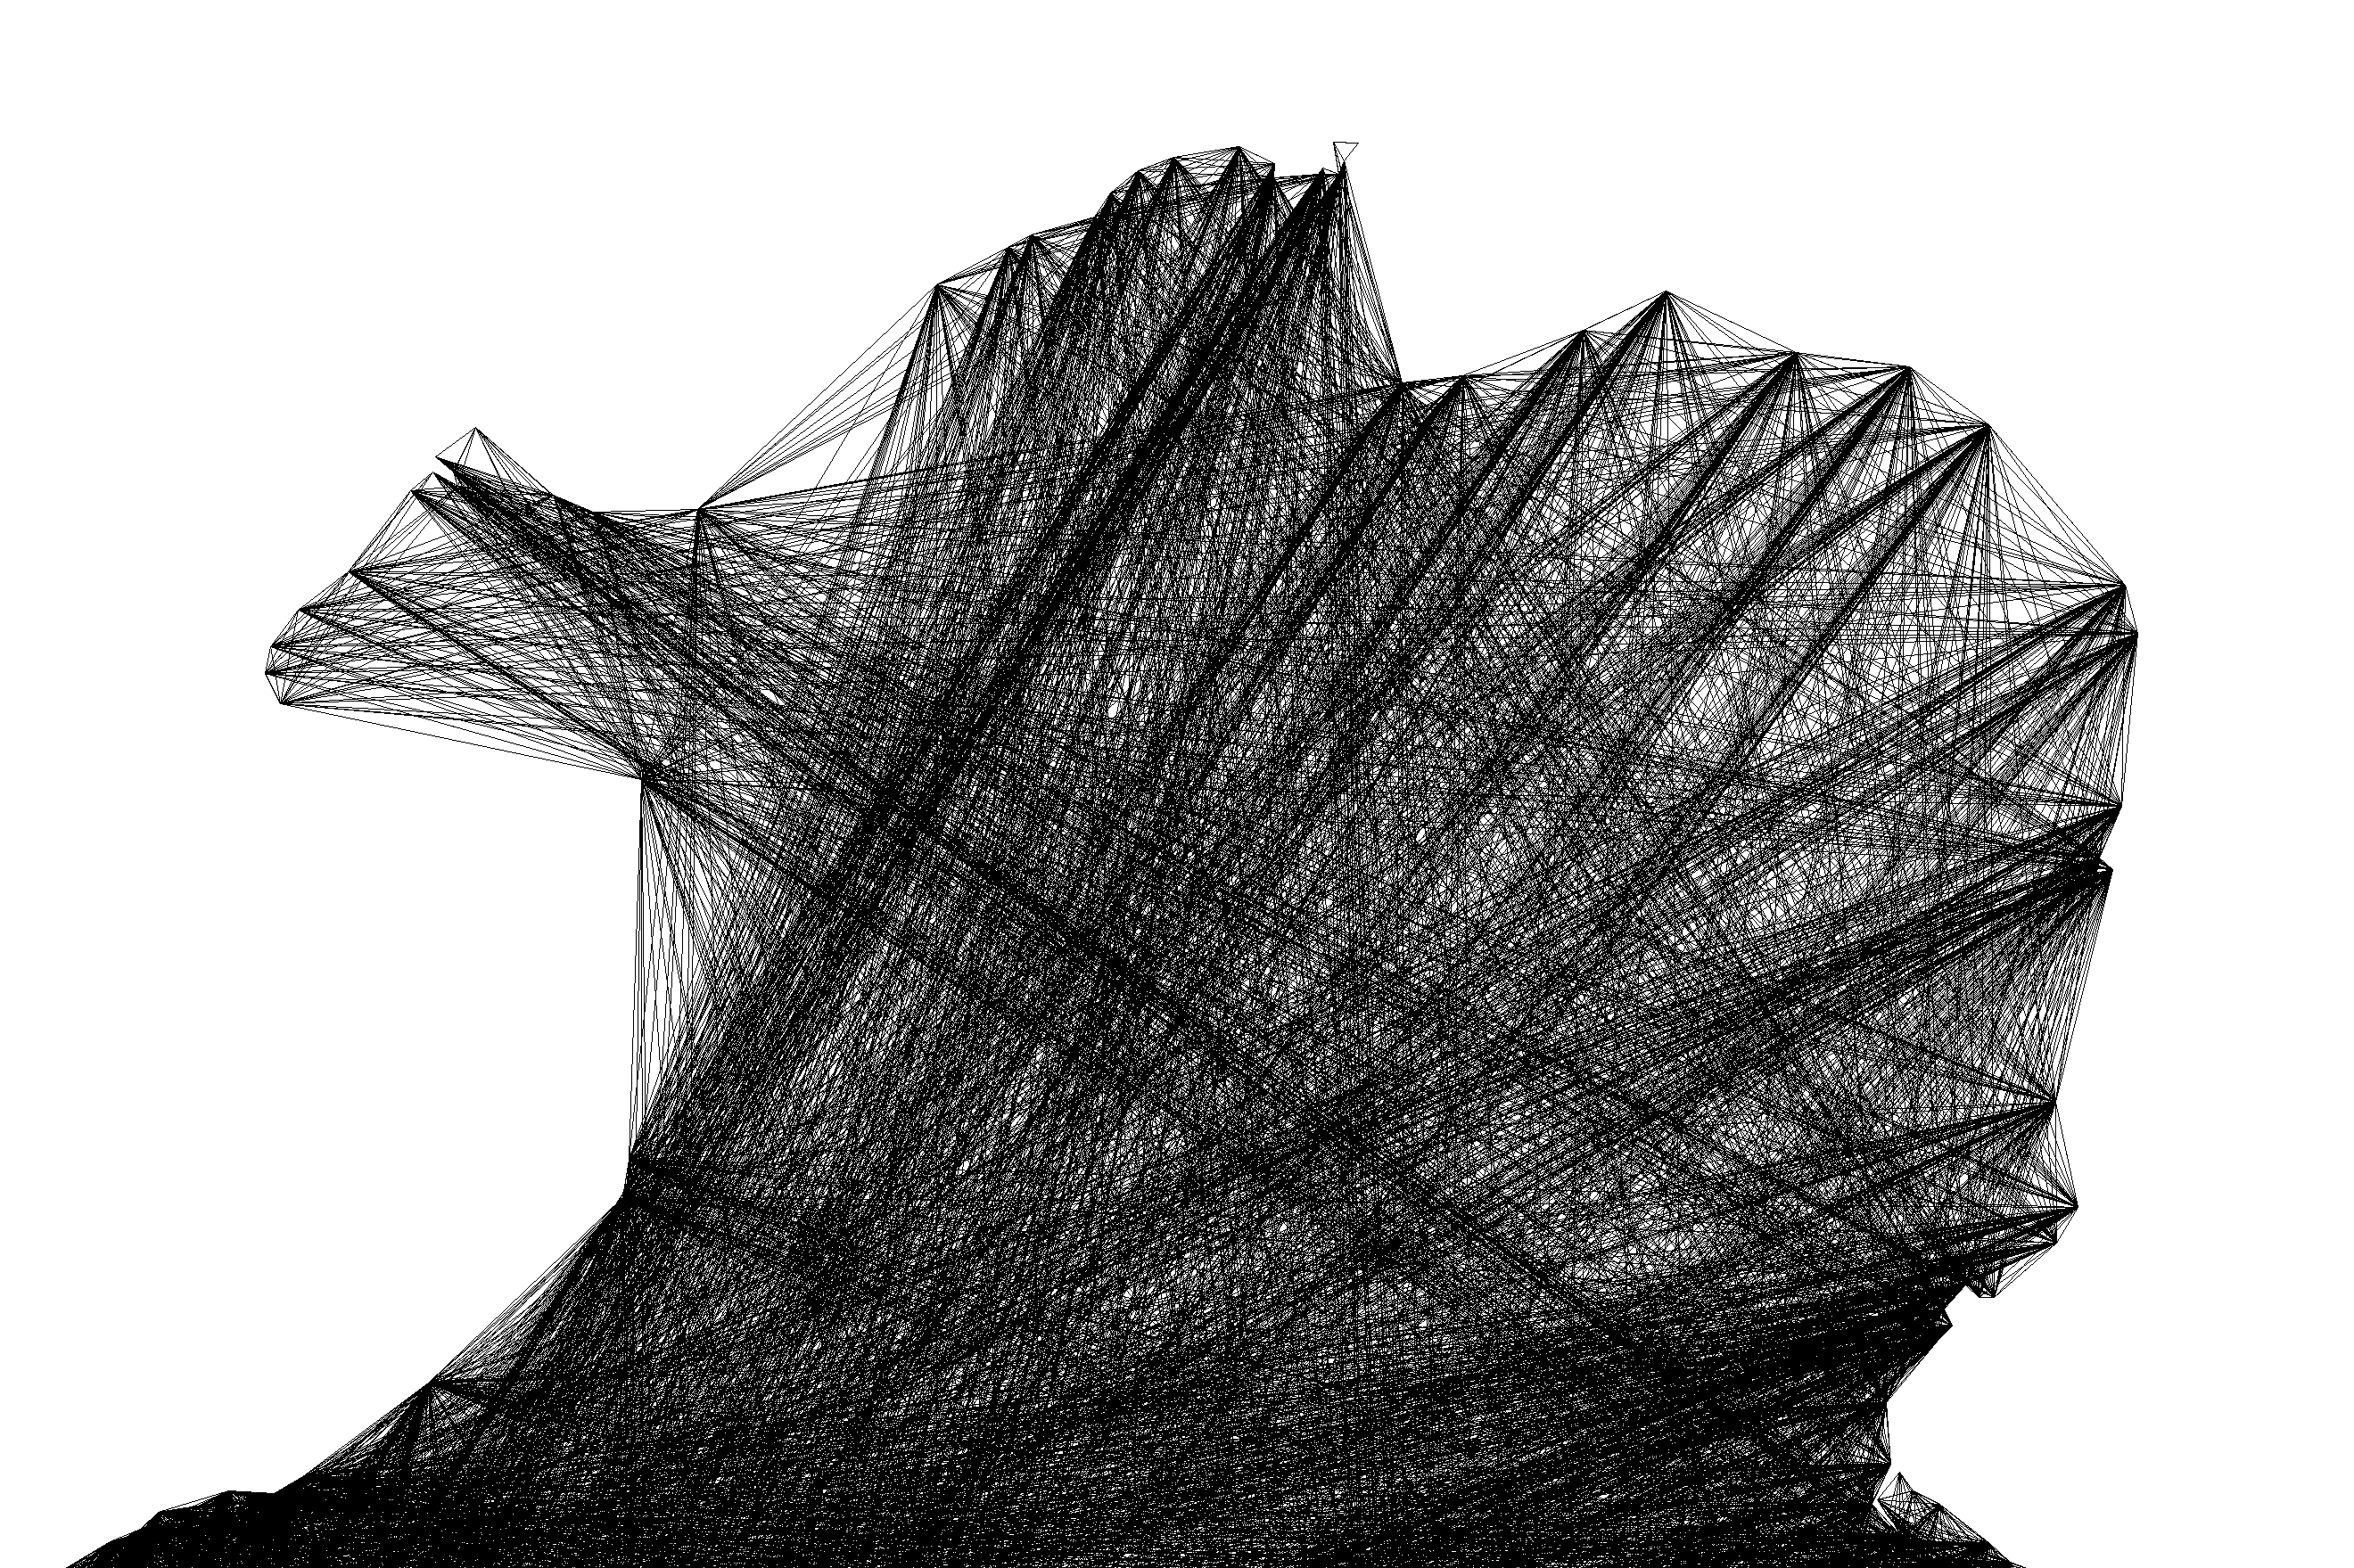
\includegraphics[width=.5\linewidth]{img/thessaloniki-visibility.png}
  \caption{Sichtbarkeitsgraph des Hafens von Thessaloniki}%
  \label{fig:thessaloniki-visibility}%
\end{figure}


\section{Speedup-Techniken}

Der \emph{Speedup} bezeichnet das Verhältnis der durchschnittlichen Laufzeit einer Dijkstra-Suche zur durchschnittlichen Laufzeit der betrachteten Methode.
Die beiden betrachteten Speedup-Techniken zum Finden kürzester Pfade benötigen eine Phase der Vorbehandlung (\emph{Preprocessing}), damit danach kürzeste Pfad Anfragen (\emph{Queries}) schneller beantwortet werden können.

Die für das Preprocessing benötigte Rechenzeit und der zusätzlich benötigte Speicher sollten in einem sinnvollen Verhältnis zum Speedup und zur Anzahl der Anfragen stehen.
Ist der Speedup hoch oder sollen viele Anfragen bearbeitet werden, so lohnt es sich, mehr in das Preprocessing zu investieren.
\autoref{fig:einleitung:preprocessing_to_query} zeigt das erwartete Verhältnis der Vorbehandlungs- zu Anfragezeiten von Contraction Hierarchies und Hierarchical Hub Labeling.

\begin{figure}[h!]
  \centering
  \begin{tikzpicture}[scale=1.5]
    % Draw axes
    \draw [<->,thick] (0,5) node (yaxis) [above] {Anfragezeit}
    |- (5,0) node (xaxis) [right] {Vorbehandlungszeit};


    \fill[black] (1, 4) circle (1pt);
    \node[right] at (1, 4) {Dijkstra};

    \fill[black] (2, 3) circle (1pt);
    \node[right] at (2, 3) {Contraction Hierarchies};

    \fill[black] (3, 2) circle (1pt);
    \node[right] at (3, 2) {Hierarchical Hub Labeling};

    \fill[black] (4, 1) circle (1pt);
    \node[right] at (4, 1) {Table Lookup};
  \end{tikzpicture}
  \caption{Verhältnis von Vorbehandlungszeit zu Anfragezeiten. Übernommen von John Lazarsfeld\cite{Lazarsfeld}}
  \label{fig:einleitung:preprocessing_to_query}
\end{figure}